\documentclass[10pt,conference]{IEEEtran}
\usepackage[T1]{fontenc}
\usepackage{amsmath,amssymb,booktabs,array,url,tikz}
\usetikzlibrary{arrows.meta,positioning}
\usepackage[hidelinks]{hyperref}
\pdfinfoomitdate=1
\pdftrailerid{}
\pdfsuppressptexinfo=15
\hypersetup{pdfauthor={Xin Xu and Jun Yu},pdftitle={An Auditable Tool for API-Derived Skill Classification}}
\title{An Auditable Tool for API-Derived Skill Classification}
\IEEEoverridecommandlockouts
\author{
\IEEEauthorblockN{Xin Xu}
\IEEEauthorblockA{Department of Automation\\
University of Science and Technology of China\\
Hefei, Anhui, China\\
xuxin123122@mail.ustc.edu.cn}
\and
\IEEEauthorblockN{Jun Yu\textsuperscript{*}}
\IEEEauthorblockA{Department of Automation and\\
Institute of Advanced Technology\\
University of Science and Technology of China\\
Hefei, Anhui, China\\
harryjun@ustc.edu.cn}
\thanks{*Corresponding author: Jun Yu (harryjun@ustc.edu.cn).}
}
\newcommand{\clogit}{\operatorname{logit}_{\epsilon}}
\begin{document}
\maketitle
\begin{abstract}
We present a multi-label tool that predicts API-derived skill annotations from an issue's title, description, and repository name. An audit of the released annotation construction motivates a conditional mapping between observed API contributions and published labels. The tool combines lexical and pretrained representations, supervised CodeBERT features, observed-skill neighbors, trees, and repository priors, while excluding query labels and PR lineage from inference. On 7,154 records under retrospective component-grouped fivefold development, micro-F1 is 0.614366 versus 0.567931 for a matched Random Forest. The final conditional-selection step adds only 0.000209 over the preceding strong policy; macro-F1 is 0.113833 and low-support labels remain undetected. Training-only baselines, controlled ablations, and unsuccessful extensions bound the contribution claims. Inference portability and one-role rebuilding are verified, but complete training reproduction, public release, and organizer-defined evaluation remain incomplete. These are internal development results, not official qualification or independent test scores.
\end{abstract}
\begin{IEEEkeywords}
issue classification, API-derived skills, multi-label learning, weak supervision, auditability
\end{IEEEkeywords}

\section{Task and Contribution}
SkillScope associates APIs used in resolving issues with skill domains and subdomains~\cite{skillscope,tagissue}. The NLBSE 2027 Skill Classification competition asks for a multi-label prediction vector~\cite{competition,repository}. Our operational target is agreement with the released annotations, not recovery of human-validated skill requirements.

The pinned issue table contains 7,154 rows and 217 count-valued labels, binarized by positive counts in release order. We retain 75 columns with no positive example. Own-repository API evidence is available for 3,070 rows and unavailable for 4,084. The snapshot has 12 repository values; the public description names 11 repositories and 7,245 merged PRs. We preserve these differences rather than silently change the dataset or assume an official split.

The contribution is an auditable tool with (i) an explicit model of its observed target construction, (ii) a strict runtime boundary and portable frozen artifact, and (iii) an evaluation separating system gains, small incremental effects, and failure cases. We do not attribute the complete RF contrast to the conditional formula.

Strong fine-tuned language models warrant explicit comparison~\cite{survey}. DENN addresses embedding and confidence biases in nearest-neighbor multi-label classification~\cite{denn}; CbMLC addresses noisy label dependencies~\cite{cbmlc}. CCMN's basic formulation assumes known class-conditional noise rates~\cite{ccmn}. Our aggregation audit does not identify latent clean skills or those rates. The bounded comparisons below do not establish superiority over these frameworks.

\section{Tool and Annotation Model}
\subsection{Legal inputs and observed contributions}
The API accepts exactly three string fields: \texttt{issue text}, \texttt{issue description}, and \texttt{Repo Name}. Extra fields, including labels and PR identifiers, are rejected. Inference reads no query API annotation, observation flag, actual patch, peer outcome, or training database. Unknown repositories use saved global fallbacks; empty batches return no predictions.

Let $M_i$ indicate an available own-row API observation and $A_{ij}$ its observed proxy for label $j$. Define $S_{ij}=M_iA_{ij}$, the row's \emph{observed contribution}. Missing evidence contributes nothing to this definition; it does not establish absence of a latent skill. Let $F_{ij}$ be the OR of the other observed contributions in the same released PR-number bag. Audited training roles satisfy
\begin{equation}
Y_{ij}=S_{ij}\lor F_{ij}. \label{eq:or}
\end{equation}
The release can associate a PR number across repositories even though PR numbers are repository-scoped. This is an annotation mechanism, not evidence that all bag members require the same skills. Unobserved latent labels remain unidentifiable from this OR constraint alone.

\begin{figure}[t]
\centering
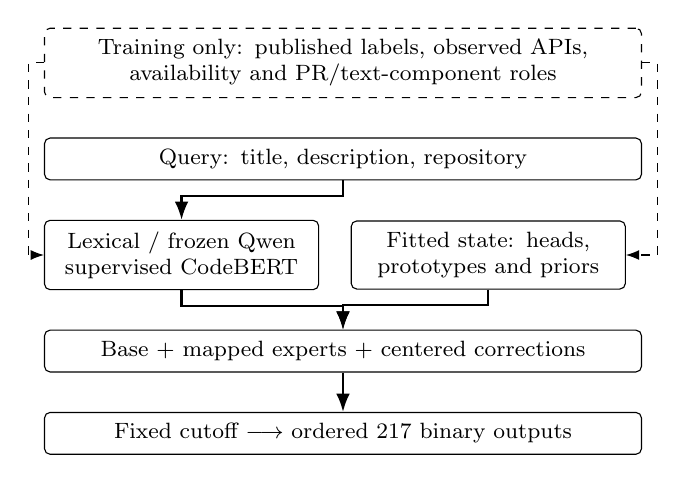
\begin{tikzpicture}[font=\footnotesize,>=Latex,
box/.style={draw,rounded corners=2pt,align=center,inner sep=4pt},
flow/.style={->,thick}]
\node[box,text width=7.3cm,dashed] (train) {Training only: published labels, observed APIs,\\availability and PR/text-component roles};
\node[box,text width=7.3cm,below=5mm of train] (input) {Query: title, description, repository};
\node[box,text width=3.2cm,below=5mm of input.south west,anchor=north west] (repr) {Lexical / frozen Qwen\\supervised CodeBERT};
\node[box,text width=3.2cm,right=4mm of repr] (state) {Fitted state: heads,\\prototypes and priors};
\node[box,text width=7.3cm,below=5mm of repr.south west,anchor=north west] (mix) {Base + mapped experts + centered corrections};
\node[box,text width=7.3cm,below=5mm of mix] (output) {Fixed cutoff $\longrightarrow$ ordered 217 binary outputs};
\draw[flow] (input.south) -- ++(0,-2mm) -| (repr.north);
\draw[flow] (repr.south) -- ++(0,-2mm) -| (mix.north);
\draw[flow] (state.south) -- ++(0,-2mm) -| (mix.north);
\draw[flow] (mix) -- (output);
\draw[->,dashed] (train.east) -- ++(2mm,0) |- (state.east);
\draw[->,dashed] (train.west) -- ++(-2mm,0) |- (repr.west);
\end{tikzpicture}
\caption{Inference boundary. Labels and lineage fit model state; they are not query inputs. The diagram does not claim fully nested estimation of every historical training centre.}
\label{fig:boundary}
\end{figure}

The bank retains training-derived labels as fitted state, as in a nonparametric classifier. Fit/query roles exclude shared PR/text components, and exported neighbor/prior components remove group and PR indices. These properties do not establish official eligibility or the organizers' interpretation of auxiliary training data.

Field types are validated before dispatch. Encoders open local assets offline with remote model code disabled. Tokenizers and fitted models are not updated from incoming batches, and an unseen repository cannot trigger query-time fitting.

\subsection{Representations and expert fitting}
The base combines title/body TF-IDF, frozen Qwen3-Embedding-0.6B vectors, and repository-shrunk published-label priors. Skill experts concatenate CodeBERT's 768-dimensional vector with two frozen Qwen3-Embedding-4B vectors of 2,560 dimensions each~\cite{codebert,qwen}, yielding 5,888 dimensions. Qwen encodes each field separately within 512 tokens; CodeBERT packs title and description into one 512-token sequence. The base Qwen uses FP32; auxiliary Qwen uses BF16, fixed left padding, mask-derived positions, last-token pooling and normalization. CodeBERT uses masked mean pooling; model identities are pinned.

The production CodeBERT learns binary API-proxy targets only on observed fit rows, with BCE, dropout 0.1, AdamW encoder/head learning rates $2\!\times\!10^{-5}/10^{-3}$, weight decay 0.01, batch 8/effective 32, seed 1234, and 10\% warmup then cosine decay. Training uses BF16 autocast with FP32 master weights; feature extraction uses FP32. The development source saves epochs 2/4/8 on an eight-epoch schedule; the full-data export uses a distinct four-epoch checkpoint.

Neighbor weights are $\max(\cos(z_i,z_n),0)^4$ for unit vectors. Up to 20 same-repository observed prototypes are used, with global fallback if none exist. The proxy vote is
\begin{equation}
q_j(X,r)=\frac{\sum_{n\in\mathcal N_i}w_{in}A_{nj}+\pi_j(r)}
                  {\sum_{n\in\mathcal N_i}w_{in}+1}, \label{eq:vote}
\end{equation}
where $\pi_j(r)$ shrinks toward the fit-global proxy mean with strength 20. Fit constants are restored. A tree expert uses a fit-only 128-dimensional SVD and a 256-tree ExtraTrees regressor, depth 12, leaf size 5, seed 1193. Its proxy outputs pass through fit-derived proxy-to-release conditional rates. The full-data bank contains 3,070 prototypes; development banks are role-specific.

\subsection{Conditional mapping and corrections}
Write $s_j=P(S_j=1\mid X,r)$ and $h_j=P(F_j=1\mid S_j=0,X,r)$. Equation~\eqref{eq:or} gives
\begin{equation}
P(Y_j=1\mid X,r)=s_j+(1-s_j)h_j. \label{eq:identity}
\end{equation}
We approximate $s_j$ by $a(X,r)q_j(X,r)$ and $h_j$ by repository rate $f_{0j}(r)$:
\begin{equation}
\widehat p_j=f_{0j}(r)+[1-f_{0j}(r)]a(X,r)q_j(X,r). \label{eq:map}
\end{equation}
The identity requires no $S/F$ independence; the plug-in approximations need not be calibrated or transport across annotation mechanisms.

Availability $a$ is L2 logistic regression ($C=1$, liblinear, seed 42), predicting fit-row $M$ from normalized title/body TF-IDF, fit-repository indicators and frozen 4B vectors. Intercepts match fit observation rates with repository shrinkage 20. Conditional-neighbor centre probabilities use grouped subfits and their own calibration; query $M$ is never supplied.

Let $N_{0j}$ count fit rows with $S_j=0$ and $C_{0j}$ those also having $F_j=1$. With $g_j=(C_{0j}+0.5)/(N_{0j}+1)$,
\begin{equation}
f_{0j}(r)=\frac{C_{r0j}+20g_j}{N_{r0j}+20}. \label{eq:prior}
\end{equation}
Absent repositories use the global rate; a zero global conditional denominator uses the fit peer mean. A centre subtracts its \emph{whole component} from counts and published-label constants.

Expert mixture $m$ modifies base probability $b$ through
\begin{equation}
\sigma\!\left(\clogit(b_j)+\lambda v(r)
 [\clogit(m_j)-\clogit(\mu_j(r))]\right), \label{eq:residual}
\end{equation}
using fit-centre expectation $\mu$, coverage weight $v$, and clipping $\epsilon=10^{-5}$. A publication correction estimates $c_j=(1-a)\gamma_{r0j}+a\gamma_{r1j}$ from shrunk fit rates $\gamma_{rmj}=P(Y_j=1\mid M=m,r)$, then applies the same centered-logit form. It models observation cohorts, not latent truth. Source expert choices/strengths are retained per fold; the full export selects equal tree/conditional-neighbor mass and residual strength 0.5.

Neighbor banks and count centres exclude whole components. Some source encoder, vocabulary, projection and correction-centre sharing remains: the full pipeline is \emph{not fully nested}.

\section{Evaluation and Bounded Follow-ups}
\subsection{Roles, selection, and fivefold results}
Components connect shared PR numbers or cleaned duplicate text. Internal fivefold development predicts each of 7,154 rows once in held roles. Three grouped inner folds choose candidate/reference within each outer training role, with ties retaining reference. All five choices lock before validation calibration. Validation searches distinct score breakpoints in $[0.05,0.95]$, maximizing micro-F1 subject to precision, recall and micro-F1 not below matched RF; ties prefer precision then a higher cutoff. With no feasible improvement it falls back to RF. All five thresholds lock before new held predictions.

This order does not remove repeated historical development effects~\cite{cawley}. RF matches roles/records; it is an internal reference, not the organizers' unresolved final baseline. We separate it from the historical wrapper fitting TF-IDF and MLSMOTE before holdout selection~\cite{repository}.

\begin{table}[t]
\caption{Frozen internal fivefold results (7,154 rows, 217 labels), not official scores. Macro-F1 uses zero-division value 0.}
\label{tab:fivefold}
\centering\small
\begin{tabular}{@{}lrrrr@{}}
\toprule
Method & Precision & Recall & Micro-F1 & Macro-F1\\
\midrule
Matched RF & .685467 & .484802 & .567931 & .108967\\
Tree/NN & .686178 & .555820 & .614158 & .113847\\
Fixed cond. & .686047 & .555920 & .614166 & .113592\\
Selected cond. & .686059 & .556240 & .614366 & .113833\\
\bottomrule
\end{tabular}
\end{table}

The system gains \textbf{4.64356 F1 percentage points} over RF, mainly through recall; precision gains only \textbf{0.05915 points}. Conditional selection adds \textbf{0.02087 F1 points} over tree/NN. Training selects it only in folds 0/4; the fixed all-fold mapping adds merely 0.000008689 absolute F1. It is not a uniformly superior replacement.

For 5,000 paired resamples of frozen predictions, the component-based descriptive 95\% precision-difference interval versus RF is $[-0.2688,0.3863]$ percentage points; the repository interval is $[-0.3716,0.4590]$. The selected-versus-tree/NN F1 interval is $[0.0000397,0.0003796]$ in absolute F1 for component resampling. These omit retraining and historical selection uncertainty, and do not prove significance or non-inferiority after search. Matched whole-tool multi-seed variance remains unmeasured.

\subsection{Label coverage}
On 142 labels with positives, selected-policy diagnostic macro-F1 is 0.173957. This does not replace the 217-label scope: all 75 globally empty labels receive F1 0 and incur no FP. Even on positive labels, coverage is limited. Table~\ref{tab:tail} assigns each held sample-label decision using that fold's \emph{fit} frequency. Low-support groups have no TP. Micro gains do not establish broad label coverage; selected conditional slightly lowers macro-F1 versus tree/NN.

\begin{table}[t]
\caption{Selected policy's frozen fivefold counts by per-fold fit support. Bins partition held decisions, not globally selected labels.}
\label{tab:tail}
\centering\small
\begin{tabular}{@{}lrrr@{}}
\toprule
Fit positives for label & TP & FP & FN\\
\midrule
0 & 0 & 0 & 48\\
1--9 & 0 & 0 & 75\\
10--49 & 0 & 0 & 444\\
$\geq50$ & 133684 & 61174 & 106084\\
\bottomrule
\end{tabular}
\end{table}

\subsection{Training-only baselines and controlled ablations}
Follow-ups use one outer fold's \textbf{4,640-row training pool}, with three component inner roles. OOF predictions also support selection/calibration: Table~\ref{tab:pilot} is pilot evidence, not fivefold test performance. No new outer predictions were produced.

Direct-$Y$ CodeBERT trains on all released-label fit rows, not only observed proxies. We compare encoder rates $10^{-5}/2\!\times\!10^{-5}$ and epochs 2/4/8, retaining the eight-epoch horizon and head rate $10^{-3}$. A separately locked repository control mixes 0.3 text probability with 0.7 fit-only Repo20 prior. Selected text uses LR$2\!\times\!10^{-5}$/epoch2; selected mixture uses LR$10^{-5}$/epoch4.

A positive BCE weight $\operatorname{clip}(\sqrt{(n_-+.5)/(n_++ .5)},1,10)$ uses fit counts only and is paired with unweighted LR$2\!\times\!10^{-5}$/epoch2. Raw and inverse weighted-risk probability $p=s/[w(1-s)+s]$ are reported. Neither improves paired micro-F1; fit-support 1--49 yields TP 0/FN 636 at the constrained cutoff and at 0.5. This is the training pool, not Table~\ref{tab:tail}.

\begin{table}[t]
\caption{Training-only pilot micro-F1 (4,640 rows). Arms use the same RF-constrained cutoff procedure. Paired loss comparisons fix LR/epoch; removals retain source centres and scales.}
\label{tab:pilot}
\centering\small
\begin{tabular}{@{}lr@{}}
\toprule
Pilot / ablation & Micro-F1\\
\midrule
\multicolumn{2}{@{}l}{\emph{Direct released-label baselines}}\\
CodeBERT, text, selected & .609213\\
CodeBERT + Repo20, selected & .613513\\
CodeBERT + Repo20, paired recipe & .612618\\
Paired + weighted BCE, raw & .612215\\
Paired + weighted BCE, corrected & .612400\\
\midrule
\multicolumn{2}{@{}l}{\emph{Tree $\times$ mapping factorial (residual 0.5)}}\\
Tree + original NN map & .617661\\
Tree + conditional NN map (control) & .617881\\
No tree + original NN map & .617311\\
No tree + conditional NN map & .617899\\
\midrule
\multicolumn{2}{@{}l}{\emph{Other removals from the control}}\\
No CodeBERT in skill vectors & .616100\\
No Qwen4 in skill vectors & .617692\\
No publication correction & .617361\\
No coverage weighting & .617003\\
\bottomrule
\end{tabular}
\end{table}

Representation deletion renormalizes remaining vectors and refits SVDs, four forests and NN banks per role, rather than zeroing old-tree inputs. Qwen4 remains in availability: skill-vector removal is not whole-encoder removal or measured memory saving. No-tree conditional differs by only 0.00001775 F1, insufficient to replace the frozen model. These one-pool studies do not isolate every upstream choice or complete full-protocol PLM/DENN comparisons.

A conditional-$h$ linear text residual failed its training-only information gate: Brier worsened from 0.070793 to 0.071597 and log loss from 0.223966 to 0.226216. No main-F1 expansion followed. Separately, eight gradient-free head/FFN edits tested rank-one reversals of late-checkpoint drift and a mean-preserving head projection in a direct-$Y$ role model. Choices used 896 development rows, then 650 confirmation rows at cutoff 0.5. Confirmation F1 changed from 0.613593 to 0.613597 for the selected head edit (precision/AP fell), and to 0.612436 for the FFN edit. Random/scale controls were retained; no edit was adopted. This was historically exposed data, not a new independent test.

\section{Artifact, Reproduction, and Limits}
The 7,154-row export has its own threefold training-OOF F1, 0.609559 (prior full model: 0.609131). This separate fit has no independent test score; evaluating it on overlapping training rows is invalid.

\begin{table}[t]
\caption{Current artifact evidence. Passing checks establish implementation or bounded reproduction, not independent predictive validity.}
\label{tab:artifact}
\centering\small
\begin{tabular}{@{}>{\raggedright\arraybackslash}p{.45\columnwidth}>{\raggedright\arraybackslash}p{.47\columnwidth}@{}}
\toprule
Scope & Status \\
\midrule
Data-root reconstruction & Rebuilt from pinned SQLite \\
One active development role & 201 tensors / 1,024 trees matched \\
Raw inference migration & 8 raw + 2 synthetic cases; corpus/network denied \\
Local source migration & 39 synthetic tests passed \\
Complete training/selection/export & Not fully rebuilt \\
Official evaluation / public release & Unverified / unpublished \\
\bottomrule
\end{tabular}
\end{table}

The CLI verifies the bundle hash before deserialization and relocates only encoder paths in memory. It returns the unchanged ordered 217 labels and binary vectors, without query-batch aggregation. Isolated inference reproduced binary outputs on eight raw cases plus two synthetic known/unseen-repository cases while denying original source/corpus/cache and network access. These check behavior, not generalization. Local packaging passed 39 synthetic tests in a separate unpack directory.

Data-root and one fixed development-role rebuilding have executed from pinned inputs/declared assets: 201 checkpoint tensors and 1,024 trees matched, with active scores differing at most $3.34\times10^{-16}$. The continuation explicitly reused a hash/text-identity-verified frozen Qwen4 input transform. Remaining roles and complete selection/calibration/export have \emph{not} all been rebuilt cleanly. An ablation aggregation failed on a missing metric import; it resumed from hash-locked completed assets without refitting or changed gates, retaining the failed record.

CPU/encoder runtimes are separate. Direct-$Y$ training's measured worker peak was 3.763 GiB allocated, not full-tool inference peak. Sequential inference reserves 11,000 MiB, not a measured end-to-end requirement. Source and frozen assets are hosted at the repository below; its Release provides hash-checked fragments. Both currently require repository authorization and are not a public artifact. Fresh installation, organizer-hardware latency and redistribution review remain gaps.\par\begingroup\raggedright\noindent Repository: \url{https://github.com/XX123122/NLBSE2027-SkillClassification}\par\noindent Assets: the repository\textquotesingle s \texttt{v0.1.0-private} Release.\par\endgroup

% Balance the final two columns at a paragraph boundary, without changing type or margins.
\newpage
The CPU runtime uses Python 3.11/NumPy 1.26.4/scikit-learn 1.5.2; encoding uses Python 3.12.3/NumPy 2.5.2/torch 2.10.0+cu130/transformers 5.15.0. These observed versions do not establish fresh-install reproducibility. The 24-role planning interface is not a complete all-role training runner.

Weak targets, cross-repository aggregation, repository transport assumptions, shared centres, adaptive development and unmeasured whole-tool seed variance limit interpretation. Diagnostics do not identify true skills or justify changing official targets. At our Nov.~16, 2026 check, the organizer TODO still leaves the formal split, 217/142 scoring scope and final baseline unresolved~\cite{repository}. Eligibility requires no decline in precision, recall or micro-F1~\cite{competition}; the narrow internal margin does not establish qualification.

We freeze the existing model after non-upgrading follow-ups. Release still needs complete reproducible training/tuning/evaluation, versioned licensed assets and organizer-protocol alignment. Rebuilding establishes reproducibility, not prospective generalization.

\begin{thebibliography}{11}
\bibitem{competition} M. Mock et al., \lq\lq The NLBSE'27 Tool Competition and Challenge,\rq\rq\ in \emph{NLBSE}, 2027. Organizer-provided citation; metadata provisional.
\bibitem{skillscope} B. C. Carter et al., \lq\lq SkillScope: A Tool to Predict Fine-Grained Skills Needed to Solve Issues on GitHub,\rq\rq\ in \emph{NLBSE}, 2025, pp. 9--12, doi: 10.1109/NLBSE66842.2025.00007.
\bibitem{tagissue} F. Santos et al., \lq\lq Tag that issue: applying API-domain labels in issue tracking systems,\rq\rq\ \emph{Empirical Software Engineering}, vol. 28, no. 5, art. 116, 2023.
\bibitem{codebert} Z. Feng et al., \lq\lq CodeBERT: A Pre-Trained Model for Programming and Natural Languages,\rq\rq\ in \emph{Findings of EMNLP}, 2020, pp. 1536--1547.
\bibitem{qwen} Qwen, \lq\lq Qwen3 Embedding model cards: 0.6B and 4B,\rq\rq\ checked Nov. 7, 2026. [Online]. Available: \url{https://huggingface.co/Qwen/Qwen3-Embedding-0.6B} and \url{https://huggingface.co/Qwen/Qwen3-Embedding-4B}
\bibitem{cawley} G. C. Cawley and N. L. C. Talbot, \lq\lq On Over-fitting in Model Selection and Subsequent Selection Bias in Performance Evaluation,\rq\rq\ \emph{JMLR}, vol. 11, pp. 2079--2107, 2010.
\bibitem{repository} NLBSE 2027, \lq\lq Skill Classification competition repository and Organizer TODO,\rq\rq\ checked Nov. 16, 2026. [Online]. Available: \url{https://github.com/nlbse2027/skill-classification}
\bibitem{survey} A. Scherp et al., \lq\lq Are We Really Making Much Progress in Text Classification? A Comparative Review,\rq\rq\ arXiv:2204.03954v7, 2026.
\bibitem{denn} Z. Cheng et al., \lq\lq A Debiased Nearest Neighbors Framework for Multi-Label Text Classification,\rq\rq\ arXiv:2408.03202, 2024.
\bibitem{cbmlc} W. Zhao and C. Gomes, \lq\lq Evaluating Multi-label Classifiers with Noisy Labels,\rq\rq\ arXiv:2102.08427, 2021.
\bibitem{ccmn} M.-K. Xie and S.-J. Huang, \lq\lq CCMN: A General Framework for Learning with Class-Conditional Multi-Label Noise,\rq\rq\ arXiv:2105.07338, 2021.
\end{thebibliography}
\end{document}
